
\chapter{Engagement and Attention Budgets}

\graphicspath{{Chapter2/plots/}}
\begin{quote}
    
    \textsl{In an information-rich world, the wealth of information means a  dearth of something else: a  scarcity of whatever it  is that information consumes. What information consumes is  rather obvious: it consumes the attention of its recipients. Hence a wealth of information creates a poverty of attention - Herbert Simon}\cite{simon1971designing}
    
\end{quote}
We live in an information rich world, where the notions of engagement, entertainment and social connection have all been migrated as close to the user as possible. Along with the portability of content consumption, content creation has also become a lot more portable and accessible because of the ever improving quality of handheld devices and their native cameras. In such an environment the headlining quote of Simon Herbert is ever so relevant. This wealth of information has created a poverty of attention. As a side effect, the poverty of attention has driven development of content formats that by design require low attention budgets. Examples of these could be Vine, Instagram stories, Whatsapp Stories, Facebook stories,  which allow users to create short ephemeral videos, which get deleted automatically after 24 hours. The user experiences are also designed around user experience of rapid scrolling, only to stop for a quick peek. 

In the context of this dissertation, it is interesting for me to investigate how users on social media platforms make decisions about whether to engage with a particular piece of content or not. More specifically, do specific user perceptions play a role in how they interact with content on these platforms. To that extent, I hypothesize that this decision is governed by two factors. The first is the state of \textbf{social embeddedness} of the consumer, such that being a particularly popular person increases one's chances of getting engagement on the content. The other factor is the \textbf{aesthetic and perceptive attributes} that make a content `catchy', such as an upbeat background music, presence of attractive faces, aesthetic framing of content, photographic structure and other attributes. Intuitively it seems plausible to track down the contributions of each of these factors if we can acquire a large enough data of social media content and their engagement metrics. There are several of such user generated content creation platforms that could be focused upon for this study, such as Instagram (1 billion users worldwide), Facebook (1.74 billion users) , Vine (200 Million active users as of 2016) or Snapchat (400 million  users). The scale at which these platforms function, makes modelling of how users spend their attention budgets, an interesting problem. This motivations is ever more crucial when recent studies have shown a high correlation between usage of these medias and mental health\footnote{https://www.bbc.co.uk/news/health-39955295} issue in young adults\cite{lup2015instagram,holland2017strong}

Although most user-generated video platforms have placed some form of limit on the duration or size of videos (e.g., YouTube had a 10 minute limit, which has since been softened to a `default' limit of 15 mins\footnote{\scriptsize https://techcrunch.com/2010/12/09/youtube-time-limit-2/}), the extremely short duration time limits of Vine, Shapchat, Instagram stories etc has led to the coining of a new term: \emph{micro videos}. Some media commentators have argued that the restrictions imposed by the micro video format could fundamentally change the way we communicate~\cite{bbc}. Indeed, it has been argued that Vine has had a significant cultural and technological impact far beyond its user base, generating several widely shared memes in its short lifetime\footnote{\scriptsize http://www.theverge.com/2016/10/28/13456208/why-vine-died-twitter-shutdown}, and inspiring other social media platforms to adopt this format\footnote{https://www.pewresearch.org/fact-tank/2013/06/20/instagram-vine-and-the-evolution-of-social-media/}. The makes Vine, a natural and crucial choice to study these processes on.


At the same time, as the format is still very new, virtually all major micro video platforms are experimenting with the format, making significant changes in the last year. For instance, Instagram extended the limit from 15 seconds to 1 minute\footnote{\scriptsize http://www.theverge.com/tech/2016/3/29/11325294/instagram-video-60-seconds}. Vine is undergoing a major overhaul -- Twitter recently said it would close down the Vine website and community. The new version of the Vine app retains the 6.5 second video format, but the videos will be published directly on Twitter's feed and thus more closely integrated with its social network\footnote{\scriptsize http://www.theverge.com/2017/1/5/14175670/vine-shutting-down-rebrand-download-archive}. 

In the context of these developments, it was crucial to understand how these media formats might change the landscape of user generated content. Understanding the dynamics of interactions of users with this format might have large impact when it comes to social media messaging and marketing strategies. Hence I examine this dimension of user perception of this media, along two dimensions: 
\begin{itemize}
    %\item[\textbf{RQ1}] How do micro videos differ from other user generated content (e.g., Videos on YouTube, Images on Flickr?)? 
    \item[\textbf{RQ1}] What are the relative roles of  social and content quality factors in driving engagement and popularity in micro-videos?
    \item[\textbf{RQ2}] How does the strict time limit impact video quality, and user engagement (both as creators and consumers) with such videos? %And as a corollary, do longer time limits change quality or user engagement?
\end{itemize}

I answer these questions from an empirical perspective, using a dataset of nearly all ($\approx 120,000$) Vine videos that were uploaded to one of the 18 globally available channels on Vine during an 8 week period. We complement these with other datasets including a curated dataset (\emph{POP12K}) of 12,000 popular Vine videos, as well as samples from other micro-video platforms such as Instagram.

To address \textbf{RQ1}, we take the three metrics of popularity which are collected -- counts of loops, reposts and likes -- as quantification of the \emph{collective} user engagement of the consumers of a video, and ask to what extent the content- and social network-related features affect these metrics. To answer this question, we develop a novel pipeline, that helps us understand individual influences of different features selected, on the popularity of a content item.
We train a random forest classifier that, given a threshold for a metric of popularity, is able to able to distinguish items on either side of the threshold into popular and unpopular classes  with high accuracy, precision and recall, using the features we have identified. The relative importance of different features then gives an indication of the extent to which those features affect the metric under consideration. We progressively consider higher and higher threshold values for videos to qualify as popular or engaging, and thereby identify trends and changes of relative importance of different features. Interestingly, we find that as the threshold for popularity becomes more and more stringent, features that represent quality of the content become collectively as important as social features such as the number of followers. Echoing an effect also observed in Instagram photos~\cite{bakhshi2014faces}, we find that presence of faces in vine videos significantly increases engagement, and is the most important content-related factor.

Next, to explore \textbf{RQ2} we look at how the quality of the video varies over time in micro-videos, and discover a \emph{primacy of the first second} phenomenon: the best or most salient parts of the video, whether in the aesthetic space or affect (sentiment) space, are more prevalent in the initial seconds of the micro video, suggesting that the authors are consciously or subconsciously treating micro-videos similar to images -- in the initial part, the video is composed with aesthetics and affective quality in mind, resulting in a higher quality level; but quality declines as the video plays over time. Furthermore, echoing the primacy of the first second phenomenon, we find that the quality of the first seconds of the video are as effective as the quality of the whole video in predicting popularity/engagement. Fig.~\ref{fig:Vine_samples} shows examples of these effects through two videos in our dataset of popular videos. In both videos, we observe content quality deteriorate over time, illustrating the primacy of the first seconds. 

\begin{figure}[!tbh]
    \centering
    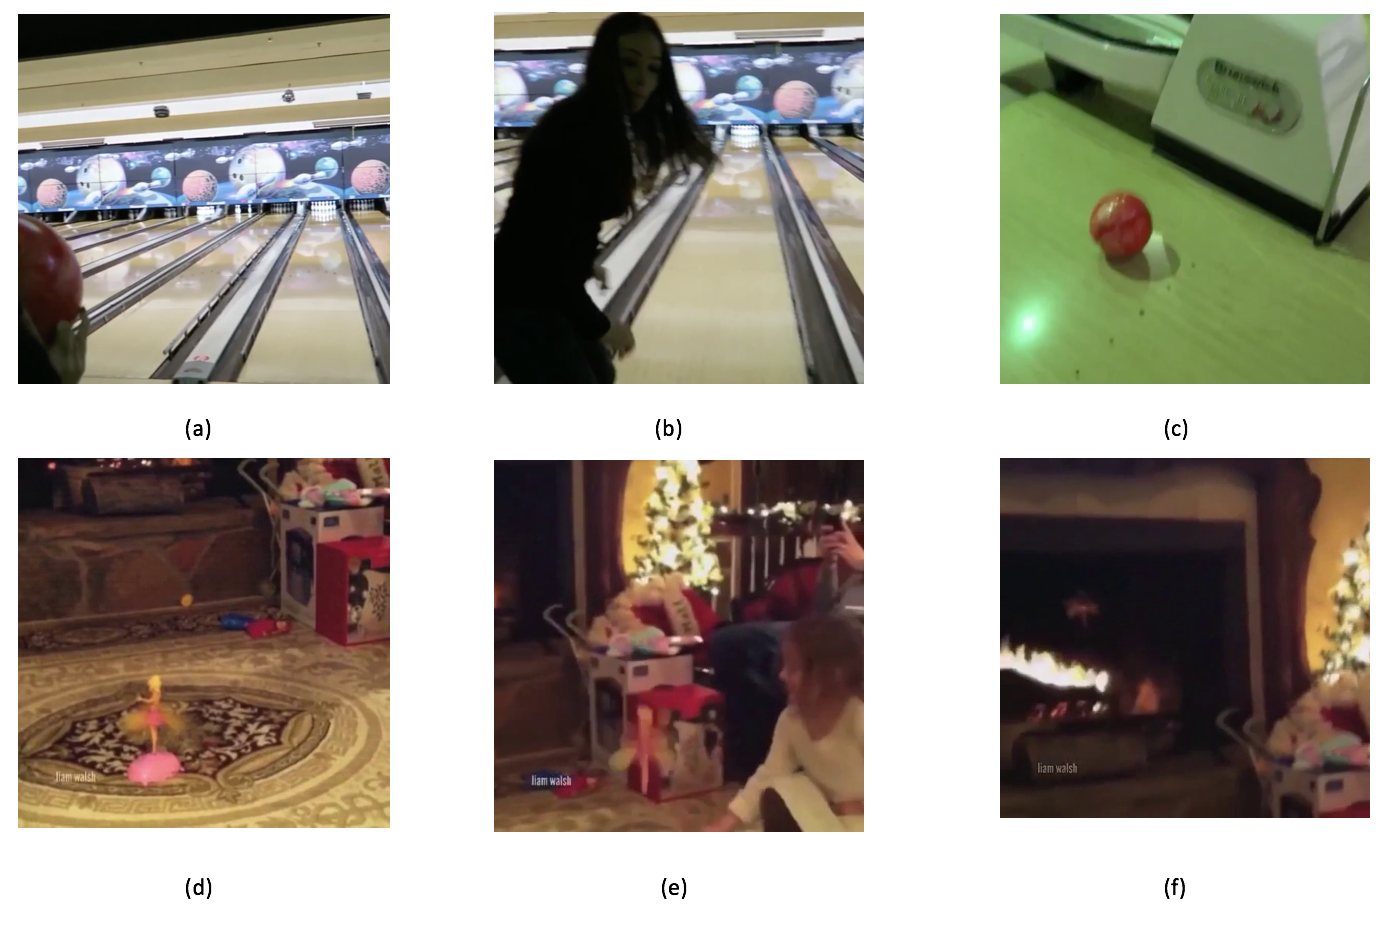
\includegraphics[width=0.7\columnwidth]{Vine_samples2.png}
    \caption{\textsl{ Vine Samples from first, second and thirds one thirds of the video. Images (a) , (b) and (c) show a progressive drop in brightness and sharpness due to shaky camera. Images (d) (e) and (f) shows a progressive drop in contrast.}}
    \label{fig:Vine_samples}
\end{figure}

We confirm these computationally acquired findings with real user impressions by designing a survey which was answered by 115 respondents: Over 66\% of users react to (like/comment on) content from their friends, making social interaction a significant part of content consumption; and 44\% of users form opinions about videos in the first few seconds, validating the observed primacy of first seconds effect. Our survey also suggests that platforms such as Vine are seen as less professional and more immediate formats than, say Flickr images or YouTube videos, providing support to David Pogue's  position that micro videos are a new kind of user-generated content~\cite{pogue13}, and therefore should be treated differently when it comes to user engagement.



\section{ Related Work}
this work closely relates to those works  in machine vision that infer intangible properties of images and videos. While  computer vision frameworks typically focus on analysing image semantics using deep neural networks \cite{krizhevsky2012imagenet}, researchers have started exploring concepts beyond semantics, such as image memorability \cite{isola2011makes}, emotions \cite{Machajdik}, and, more broadly, pictorial aesthetics \cite{datta2008algorithmic,luo2008photo,goodSelfie}. 
This work specifically focuses on on-line visual content collected from social media. Researchers have shown that, by leveraging social media data in combination with vision techniques, systems can estimate visual creativity \cite{redi20146},  sentiment \cite{wang2015inferring,jou2015visual} and sarcasm \cite{schifanella2016detecting}. %Recent studies have also shown that vision techniques can be employed to detect the ambience of the places visited by the subject of a profile picture  \cite{redi2015like}, the home and vacation location of the owner of a photo album \cite{zheng2015towards}. 

More specifically, our work closely relates to research that combines social media studies and computer vision to analyse popularity and diffusion for social media posts: for example, Zhong \textsl{et al.} were able to predict the number of post ``re-pins''  given the visual preferences of a Pinterest user \cite{predictingPintrest}; recent work \cite{Mazloom:2016:MPP:2964284.2967210} has also used multimodal features to predict the popularity of brand-related social media posts. Different from these works which focus on prediction,  this work looks at understanding user engagement. 

Media popularity prediction studies generally focus on non-visual features.  For example, \cite{Yamasaki:2014} used textual annotations to predict various popularity metrics of social photos. Social metrics such as early views \cite{pinto2013using} or latent social factors \cite{nwana2013latent} have also been used to effectively estimate video popularity. However, the fact that many popular media items may not depend on the social  network~\cite{Cha2009Flickr} suggests that intrinsic media quality is an important factor for diffusion, engagement and popularity, which we explore in this work.

Recent work in the field has explored the importance of visual content in analysing popularity: \cite{totti14impact} analysed the visual attributes impacting image diffusion,  and \cite{schifanella2015image} studied relations between image quality and popularity in on-line photo sharing platforms.  Bakhshi et al  \cite{bakhshi2014faces} showed that pictures with faces tend to be more popular than others. Similar to our work, researchers have used computer vision techniques to estimate image popularity in Flickr \cite{Khosla:2014}. Moreover, a work done by Fontanini et.al \cite{fontanini2016web} explores the relevance of perceptual sentiments to popularity of a video. 
Unlike these works, we  explore content features to fully understand user engagement and popularity in micro videos, a new form of expression radically different from both the photo medium and the video medium.% We motivate our study by providing quantitative evidence for such radical novelty introduced by Vine videos, running a cross-platform comparison study based on audiovisual features.  

Micro videos are relatively new, so work specifically on micro video analysis has been limited. Redi \textsl{et al.}~\cite{redi20146} quantify and build on the notion of creativity in micro-videos. A large dataset of 200K Vine videos was collected by Nguyen et.al \cite{nguyen2016open}, focusing on analysis of tags. Closest to our work is Chen \textsl{et al.}~\cite{Chen:2016:MTM:2964284.2964314} who use multimodal features to predict popularity in micro videos. However, although we use popularity prediction as an intermediate tool, our focus is on understanding impact and importance of different features in determining popularity or engagement. To this end, we introduce a novel methodology 
%(\S\ref{sec:methodology}) 
that allows understanding up to which point social features are prominent over content features. Additionally, we demonstrate the ``immediacy" of engagement with micro videos by showing that the content from the first two seconds of the video is just as good at predicting  popularity as the entire content 
%(\S\ref{sec:first-seconds})
. Collectively, these results allow us to characterise Vine as a new medium of expression, different from previous work.




\section{Introduction to Datasets}

Micro videos were pioneered and popularised by Vine\footnote{\scriptsize http://vine.co}, which was launched in 2012. Vine videos are constrained to a maximum length of 6.5 seconds. Videos are typically created using the mobile app and posted on user's profile which can be followed and shared by other users within the app or the website. %Instagram on the other hand, in early 2016,  introduced videos with a relaxed time duration constraint of up to 1 minute, which has seen a sudden surge in usage. 
We stress most of our work on videos sampled from Vine, complemented by %YouTube, Flickr and 
Instagram data, which will be introduced as appropriate. The rest of this section gives details about the Vine datasets.




\subsection{Dataset description}\label{sec:dataset}
\begin{table}[hbt]
    \centering
    \begin{tabular}{l|cccc}
        \thead{Dataset} & \thead{\shortstack{Posts\\ (total)}} & \thead{\shortstack{Loops/Views\\ (median)}} & \thead{\shortstack{Reposts\\ (median)}} & \thead{\shortstack{Likes\\ (median)}} \\
        \hline
        POP12K & 11448 & 318566  & 2173 & 7544  \\
        ALL120K & 122327 & 80 & 0 & 2 \\
        %INSTA15k & 14568 &  93  & N/A  &  40\\
    \end{tabular}
    \caption{Summary characteristics of datasets used}
    \label{tbl:dataset}
\end{table}


The data used in this work is summarised in Table~\ref{tbl:dataset}, and was collected in two phases as described below: 

\paragraph{Popular videos dataset} First, we collected $\approx$ 12,000  videos which have been marked by Vine as `popular', by tracking the `popular-now' channel\footnote{\scriptsize https://vine.co/popular-now} over a three week period in Dec 2015, and downloading all videos and associated metadata once every six hours, and removing any overlapping videos from the previous visit. The crawling period was chosen to ensure that consecutive crawls have an overlap of several videos, and this sufficed for all visits made to the website during the data collection period; thus the dataset we collected is a complete collection of all `popular-now' vines during the 21 days under consideration. %After removing all duplicates, a total of \textbf{XXX} popular videos were collected. 

Vine does not disclose the algorithm used to mark a Vine as popular; yet we observe (see Table~\ref{tbl:dataset}) orders of magnitude more loops, reposts and likes in the popular-now dataset than in the non-popular dataset. Thus we believe that the algorithm used by Vine to select vines for the 'popular-now' channel is strongly affected by the numbers of loops/revines/likes. Note that the numbers of loops etc. were collected at the time of crawl, within a maximum of six hours of being posted on the 'popular-now' channel, which limits the possibility that the counts increased \emph{as a result} of being featured on the popular-now channel. In the rest of the chapter, we use the counts in the popular-now dataset to calibrate the definition of `high engagement'. While there is a possibility that this is a biased proxy for global engagement, it nevertheless provides a baseline against which to compare all videos.

\paragraph{All channel videos dataset} In the second phase, we collected 
videos accessible from each of the 18 global Vine channels or categories%\footnote{https://vine.co/api/timelines/channels/<channelNumber>/recent?size=100} 
over a period of {8 weeks} from {Aug 16 to Oct 12  2016}. Again, a crawling period of six hours was chosen for consecutive visits to the same channel, and the 100 most recent vines were fetched with each visit. The number 100 was a result of an API limit from Vine. 
%As shown in Fig.~\ref{fig:download-fraction}, the  vines returned has a significant overlap with vines fetched from the previous visit. 
Our dataset captures nearly all videos uploaded to Vine and assigned to a channel. The only exception is the extremely popular comedy channel, for which we nearly always find more than 100 new videos (we only download the 100 most recent videos for the comedy channel). In total, this results in a dataset of $\approx$120,000 videos. We track  loop, revine and like counts  over time, periodically updating each video's counts every three days until the end of  data collection. At the last tracking cycle, we have metadata for each post for  3 weeks after initial  upload.

Note that while we obtain nearly all videos across the channels, our dataset does \emph{not} capture  \emph{all} videos uploaded to Vine -- Vine creators do not need to assign a video to a channel. However, due to the Vine platform structure,  vines that are not in channels have near-zero probability to get seen by other users apart from the followers. % and we do not discover any vines not in channels. 
We use channels to restrict ourselves to vines which have a chance to get exposed to a reasonably global audience of those interested in a topic category, and therefore to vines that have a higher potential for garnering high engagement. 


\subsection{Feature Descriptions}
\label{sec:features}
In order to fully understand how micro-videos engage users, we characterize the content of videos using computer vision and computational aesthetics techniques and  extract a number of features (Table ~\ref{tab:Features_table} in Appendix), which can be divided into the following categories: 

\noindent\textbf{Image quality features} These features are mostly taken from computational aesthetics literature, and have been recognized as heuristics for good photography. Prior work~\cite{predictingPintrest} has identified a set of image quality features that robustly predict user interest in images. We  adapt these to videos by computing  the features on images taken at regular intervals from the video under consideration, and use the values to understand intrinsic quality of Vine videos. We use a combination of low-level features such as contrast, colourfulness, hue saturation, L-R balance, brightness and sharp pixel proportion, together with higher level features such as simplicity, naturalness of the image, and adherence to the  ``rule of thirds'' heuristic. 

\noindent\textbf{Audio features}	
Following previous work on micro videos~\cite{redi20146}, we use audio features known to have an impact on emotion and reception. Using open source tools~\cite{lartillot2007matlab,laurier2009exploring}, we measure \emph{loudness} (overall volume of the sound track), the \emph{mode} (major or minor key), \emph{roughness} (dissonance in the sound track), and \emph{rhythmical} features describing abrupt rhythmical changes in the audio signal. 

\noindent\textbf{Higher Level features} Affect (emotions experienced) is well known to strongly impact on user engagement~\cite{o2008user,leung2009user}. To understand the sentiment conveyed by the video frames, we use the Multi Lingual Sentiment Ontology detectors~\cite{jou2015visual} which express visual sentiment of video frames on a scale of 1 (negative) to 5 (positive). We sample frames at regular intervals and compute the affect evoked by these frames using this 5-point scale. Another higher level feature we consider is the presence of faces, which has previously been shown to have a strong influence on  likes and comments in image-based social media~\cite{bakhshi2014faces}. We therefore adapt it to the video context by computing the \emph{fraction of frames with faces}. Finally \emph{Number of past posts} by the creator of the video under consideration is also included to reflect user experience and activity on the social media network.

\noindent\textbf{Social  features} We consider the \emph{number of followers} of  the author of a content as a direct feature to reflect the user's social network capital. 

A more detailed description of all the features can be seen in  Table \ref{tab:Features_table}.

\begin{table}[hp]
    \centering
    \resizebox{\linewidth}{!}{%
        \begin{tabular}{|c|r|c|p{17cm}|}
            \hline
            &  \textbf{Features} & \textbf{dim} & \multicolumn{1}{c|}{\textbf{Description}}\\
            \hline
            %    \multirow{15}{*}{\rotate{Content Features}}
            &\multicolumn{3}{c|}{\textbf{Visual Quality Features}} \\
            \cline{2-4}
            & RMS contrast & 1 & RMS contrast is calculated as standard deviation across all the pixels relative to mean intensity \\[4pt]
            &  Weber Contrast & 1 &  Weber contrast is  calculated as  $ F_\textit{weber} = \sum_{x = width}\sum_{y = height} \frac{I(x,y) - I_\textit{average}}{I_\textit{average}} $ \\[4pt]
            & Gray Contrast & 1 & Gray contrast is calculated in similar to RMS contrast in HSL colour space for the L value of pixels. \\ %[4pt]
            & Simplicity & 2 & Simplicity of composition of a photograph is a distinguishable factor that directly correlates with professionalism of the creator \cite{ke2006design}. We calculate Image simplicity by two methods: Yeh simplicity~\cite{yeh2010personalized} and Luo simplicity~\cite{luo2008photo}. \\ %[4pt]
            & Naturalness & 1 & How much does the image colors and objects match the real human perception?To compute image naturalness we convert the image into the HSV color space and  then identify pixels corresponding to natural objects like skin, grass, sky, water etc. This is done by considering pixels which an average brightness V \begin{math} \in \end{math} [20 , 80] and saturation S > 0.1. The final naturalness score is calculated by finding the weighted average of all the groups of pixels. \cite{predictingPintrest}. \\ %[4pt]
            & Colourfulness & 1 & A measure of colourfulness that describes the deviation from a pure gray image. It is calculated in RGB colour space as  
            $\sqrt{\sigma_\textit{rg}^2 + \sigma_\textit{yb}^2 } + 0.3\sqrt{\mu_\textit{rg}^2 + \mu_\textit{yb}^2}$ where $ \textit{rg} = \textit{R} - \textit{G}$ and $ yb = \frac{R + G}{2} $ and $\mu \text{ and }  \sigma $ represent mean and standard deviation respectively \\ %[4pt]
            & Hue Stats & 2 & Hue mean and variance which signifies the range of pure colours present in the image. It is directly derived from the HSL colour space \\ %[4pt]
            & LR balance &1 & Difference in intensity of pixels between two sections of an image is also a good measure of aesthetic quality. In non-ideal lighting conditions, images and videos tend to be over exposed in one part and correctly exposed in other. This is generally a sign of amateur creator. To capture this we compare the distribution of intensities of pixels in the left and right side of the image. The distance between the two distributions is measured using Chi-squared distance.\\
            & Rule of Thirds & 1 & This feature deals with compositional aspects of a photograph.This feature basically calculates if the object of interest is placed in one of the imaginary intersection of lines drawn at approximate one third of the horizontal and vertical positions. This is a well known aesthetic guideline for photographers. \\
            & ROI proportion & 1 & Measure of prominence given to salient objects. This measure detects the salient object in an image and then measures proportion of pixels its relative to the image \\
            & Image brightness & 3 & Features signify brightness of the image. Includes average brightness, saturation  and saturation variance\\
            & Image Sharpness & 1 & A measure of the clarity and level of detail of an image. Sharpness can be determined as a function of its Laplacian normalized by the local average luminance in the surroundings of each pixel, i.e. $\sum_{x, y} \frac{L(x, y)}{\mu_{xy}}$, with $L(x, y) = \frac{\partial^2I}{\partial x^2}+\frac{\partial^2I}{\partial y^2}$ where $\mu_xy$ denotes the average luminance around pixel (x, y).\\
            & Sharp Pixel Proportion  & 1 & Out of focus or blurry photographs are generally not considered aesthetically pleasing. In this feature we measure the proportion of sharp pixels compared to total pixels. We compute sharp pixels by converting the image in the frequency domain and then looking at the pixel corresponding to the regions of highest frequency \cite{yeh2010personalized}, using the OpenIMAJ \cite{Hare:2011:OIJ:2072298.2072421} tool.\\
            
            \cline{2-4}	
            &	\multicolumn{3}{c|}{\textbf{Higher Level Features}} \\
            \cline{2-4}
            & Face Percentage & 1 & Percentage of frames in a video, which have been tested positive for at-least one face. Faces detected using Viola Jones Detector \cite{viola2004robust}\\
            & Frame sentiment & 1 & Median frame sentiment of all the sampled frames from a micro video. The sentiment was calculated using the Multilingual Visual Sentiment 
            Ontology detector \cite{jou2015visual} \\
            & Past post count & 1 & Number of past posts user has uploaded prior to current one. This is a good measure of user's experience with the platform and activity.\\
            
            \cline{2-4}
            & \multicolumn{3}{c|}{\textbf{Audio Features}} \\
            \cline{2-4}
            & Zero Crossing rate & 1 & Zero crossing rate measures the rhythmic component an audio track \cite{laurier2009exploring}. It ends up detecting percussion instruments like Drums in the track\\
            & Loudness & 2 & This feature expresses overall perceived loudness as two components. Overall energy and average short time energy \cite{lartillot2007matlab}\\
            & Mode & 1 & This feature estimates the musical mode of the audio tract (major or minor). In western music theory, major modes give a perception of happiness and minor modes of sadness. \cite{laurier2009exploring} \\
            & Dissonance & 1 & Consonance and dissonance in an audio track has been shown to be relevant for emotional perception \cite{laurier2009exploring}. The values of dissonance are a calculate by measuring space between peaks in the frequency spectrum of the audio track. Consonant frequency peaks tend to be spaced evenly where as dissonant frequency peaks are not\\
            & Onset Rate & 1 & This measures the the Rhythmical perception. Onsets are peaks in the amplitude envelop of a track. Onset rate is measured by counting such events in a second. This typically gives a sense of speed to the track. \\
            \cline{2-4}
            &	\multicolumn{3}{c|}{\textbf{Social Features}} \\
            \cline{2-4}
            & Followers & 1 & Number of followers that the user posting a video has. This is the prime social feature available from the user meta-data. The number of followers directly represent the audience which are highly probably to engage with the video on upload.\\
            \hline
        \end{tabular}
    }
    \caption{Dimensionality and description of features used to describe Vine videos}
    \label{tab:Features_table}
    %        \vspace{-5mm}
\end{table}


\section{User Engagement in micro videos}
\label{sec:classifier}
We begin our analysis by devising a novel 
methodology to analyze how the previously defined features impact user engagement in micro videos (\textbf{RQ1}). Our results indicate the importance of social features for highly engaging videos, and that the presence of faces is a strong content-related feature that positively impacts user engagement.
%: We build a machine learning model that predicts  engagement with high accuracy, precision and recall. The  relative feature importances then indicate what aspects of the micro videos matter more to users. By varying the threshold of engagement, we can analyse how different features change for high and low engagement items.  %First, we discuss our experiment setup and then present the model's performance and discuss the implications: that content-related features are collectively more important than social features for engagement, and that presence of faces is the single most important content-related feature.

\subsection{Metrics and methodology}
\label{sec:methodology}

\begin{figure*}[htp]
    \centering
        \includegraphics[width=\textwidth]{pipeline.pdf}        \label{fig:pipeline}
\end{figure*}


To understand which aspects or features are important for user engagement, we need to: 1) define a metric for engagement, and 2) develop a methodology to study how the metric is influenced by different features. 

\noindent\textbf{Defining a metric for user engagement}:  In this chapter, we  use \emph{number of loops} of a micro video as a proxy for user engagement towards it\footnote{We obtained similar trends using number of reposts, but only report results with loops. Note that the loop counts of videos are highly correlated with reposts and likes. For example for videos in POP12K, $ corr(Loops,Likes) = 0.80$, $corr(Likes,Reposts) = 0.91$, $corr(Reposts,Loops) = 0.74$.}.
Although user engagement is a broadly used term, and other metrics may well be used to represent user engagement, our choice is in line with previous related social media studies (e.g.~\cite{bakhshi2014faces})  that have used social attention metrics such as likes and comments to study user engagement. Video hosting platforms like Youtube also use the number of views (similar to number of loops on Vine) as a core metric for their user engagement API\footnote{\scriptsize https://developers.google.com/youtube/analytics/v1/dimsmets/mets}. In the rest of the chapter, we will use popularity and engagement interchangeably.

\noindent\textbf{Motivating the methodology}: 
Given a set of features, if we can build a machine learning model that uses the features to predict which content items are highly engaging, the relative importance of the different features in making the prediction can tell us about the relationship between the features and engagement. However, our results will only be as `good' as the model is in predicting loop counts. Since predicting popularity with exact numbers such as loop counts is a hard problem, we turn to a simpler one: We define an arbitrary threshold count for loops, and categorize micro videos as popular or unpopular depending on whether the loop count is over or under the threshold.  We then design a classifier that predicts whether a micro videos is popular or unpopular (alternately, as engaging or not) based on our set of 28 features (Table~\ref{tab:Features_table}) . As discussed next, a simple random forest classifier can be trained to make this prediction with high precision and accuracy. The relative importance of different features then tells us about how the features affects user engagement.

This method has one major limitation: its dependence on the arbitrarily defined loop count threshold. Therefore, we conduct a  sensitivity analysis by training a series of binary classifiers for different loop count thresholds. This also allows us to study shifts in relative importance, as we move up the scale towards more popular and engaging objects, by defining increasingly higher numbers of loop counts as the threshold for categorizing a video as popular (or engaging). 

\subsection{Model details}
\label{sec:model-details}
\noindent\textbf{Setup}
%Due to the exhaustive nature of our data, the computational resources in terms of CPU usage and time would be unmanagable, so 
We sample 12,000 videos from our dataset, out of which 6,000 are popular videos from  POP12K, and 6,000 randomly sampled from the ALL120K dataset, thus representing the entire spectrum of engagement levels. In each video, we sample the video track for individual frames at every second, and extract the audio track as well as meta-data related to the video and its author. Using these, we then compute the 28 dimensional vector of all the features in Table \ref{tab:Features_table} and train a random forest classifier to distinguish popular and unpopular videos for different thresholds of popularity. We used the implementation from the \emph{SKLearn} package with $\sqrt{n_{features}}$ split and $500$ estimators, which provided the best trade-off between speed and prediction performance.

\noindent\textbf{Performance Results} 
Different classifiers are trained using the above method for different engagement/popularity thresholds, using an 80-20 split for training and validation. Fig \ref{fig:Classifier_performance} shows how these perform as we vary the threshold of ``engagement'' (popularity) from 80 loops (the median for ALL120K) to  $\approx$ 500,000 loops (1.5 times the median of the popular videos i.e., POP12K). At each training iteration with a changed ``engagement'' threshold, we re-balance the dataset by choosing equal number of samples which fall in either classes. We take care that we are training on at-least 20\% of the complete dataset by the end of the process, and stop increasing the threshold beyond that point to avoid over-fitting. The classifiers gave consistently high performance on the validation dataset (see lines labeled 6 sec), never dropping below 90\% for accuracy, and 80\% F-1 score, validating our next results about the importance of different features. 

\subsection{Feature analysis and implications}
The impact of individual features on user engagement is calculated using Gini importance~\cite{louppe2013understanding}, and combined into social-  and content-related (i.e., audio and video-related) features as described before (\S\ref{sec:features}). Fig.~\ref{fig:Feature_importance} shows the trends in  feature importance as a function of engagement threshold used (see lines labeled 6 sec). We observe that at lower thresholds of popularity, social features are much more important than content-related features, but at higher thresholds, content-related features increase in importance to become just as important as social features, suggesting that \emph{content quality is important for user engagement at the top end of engagement}. This facet of users' engagement with Vine might legitimize Twitter's decision to more closely integrate the Vine platform with its social network: since a large part of micro-video popularity can be explained with social factors, a better social network might further foster engagement with this unique form of expression. %However, it is still unclear whether this closer integration would help promoting  less popular videos  by providing an alternate route of exposure, or will  a diffusion mechanism based purely on social factors limit the access to less popular videos? 

We drill down further in Fig.~\ref{fig:Feature_importance_content}, and examine the importance of different kinds of content-related features. For each class of content-related features, we plot the mean of the feature set of the class. We observe that in terms of effective importance of different feature tracks, sentiment is the weakest influencer in the classifier decision process. We conjecture that the relative lack of importance of sentiments may partly be due to the extremely short nature of micro videos, which does not let emotional `story arcs' and plots (e.g., drama) to develop as strongly as in longer videos.
%We do this by finding the mean of a set of feature importances corresponding to a particular set of features. 
%Amongst aesthetic, the Luo Simplicity was the most dominant for 5 classifier train iterations and then colour contrast becomes dominant for the rest of the train iterations. Among the Audio features, short-time energy ,which is a measure of sudden loudness, is dominant for the first 25 train iterations . At the highly selective range , Rhythemical features or Zero crossing rate , which measure the rhythmical content of a waveform , become dominant. 


Further, we observe that the presence of faces in a frame strongly outweighs all other content-related features in predicting popularity. %\ns{document which is the dominant feature of each kind}
We confirm this in Figure~\ref{fig:Face_CDF} by comparing the percentage of faces in popular POP12K videos with the corresponding percentage in ALL120K videos (which contain a large number of unpopular videos as well as a few popular ones).  These results indicate that popular videos tend to have more faces, i.e., ``\emph{faces engage us}''. This is in alignment with similar results on other platforms, which also indicate that faces greatly enhance popularity related metrics such as likes and comments~\cite{bakhshi2014faces}. 


\begin{figure*}[htp]
    \centering
    
    \subfloat[ Content Vs Social Features ]{
        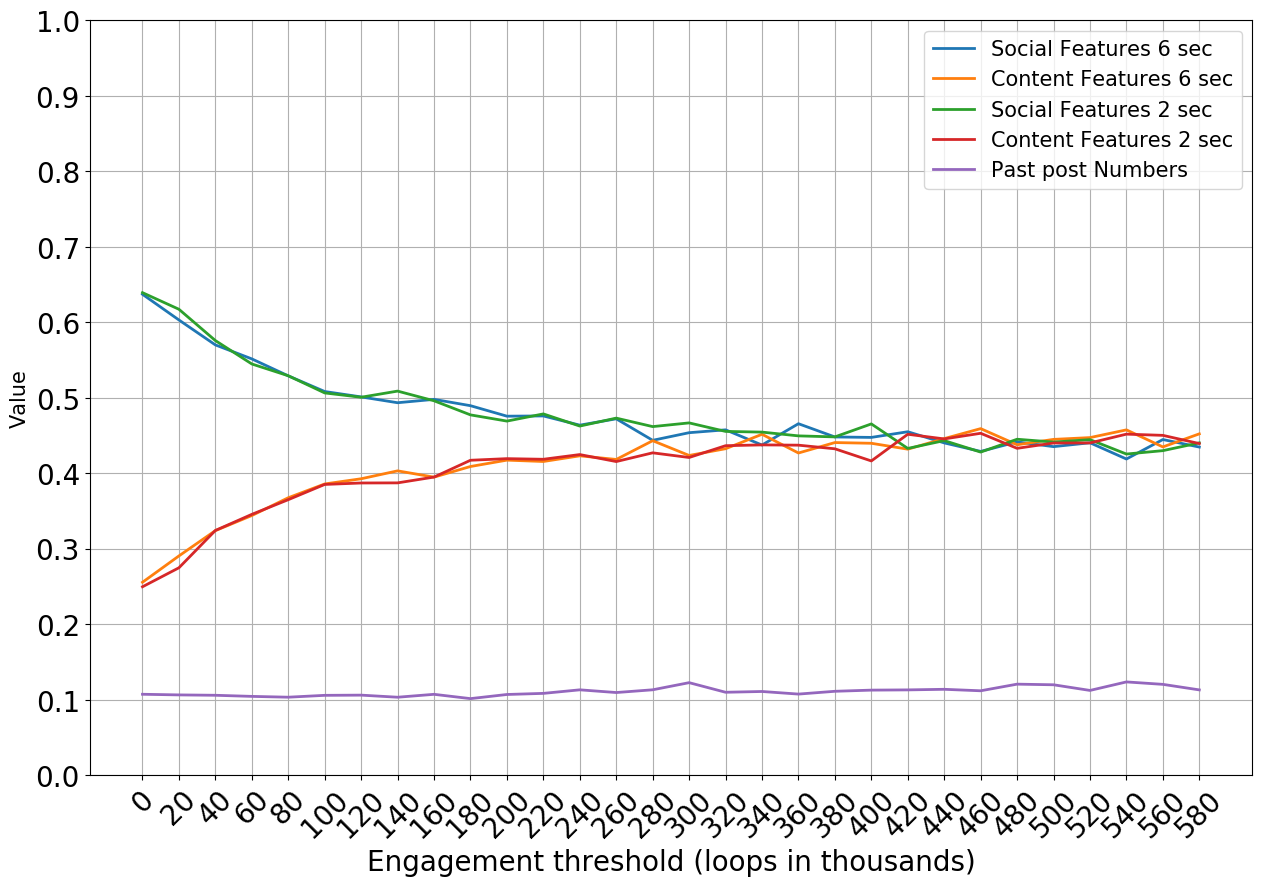
\includegraphics[width=0.5\textwidth, height = 4.5cm ]{engagement}
        \label{fig:Feature_importance}
    }
    \subfloat[ Individual Content Features ]{
        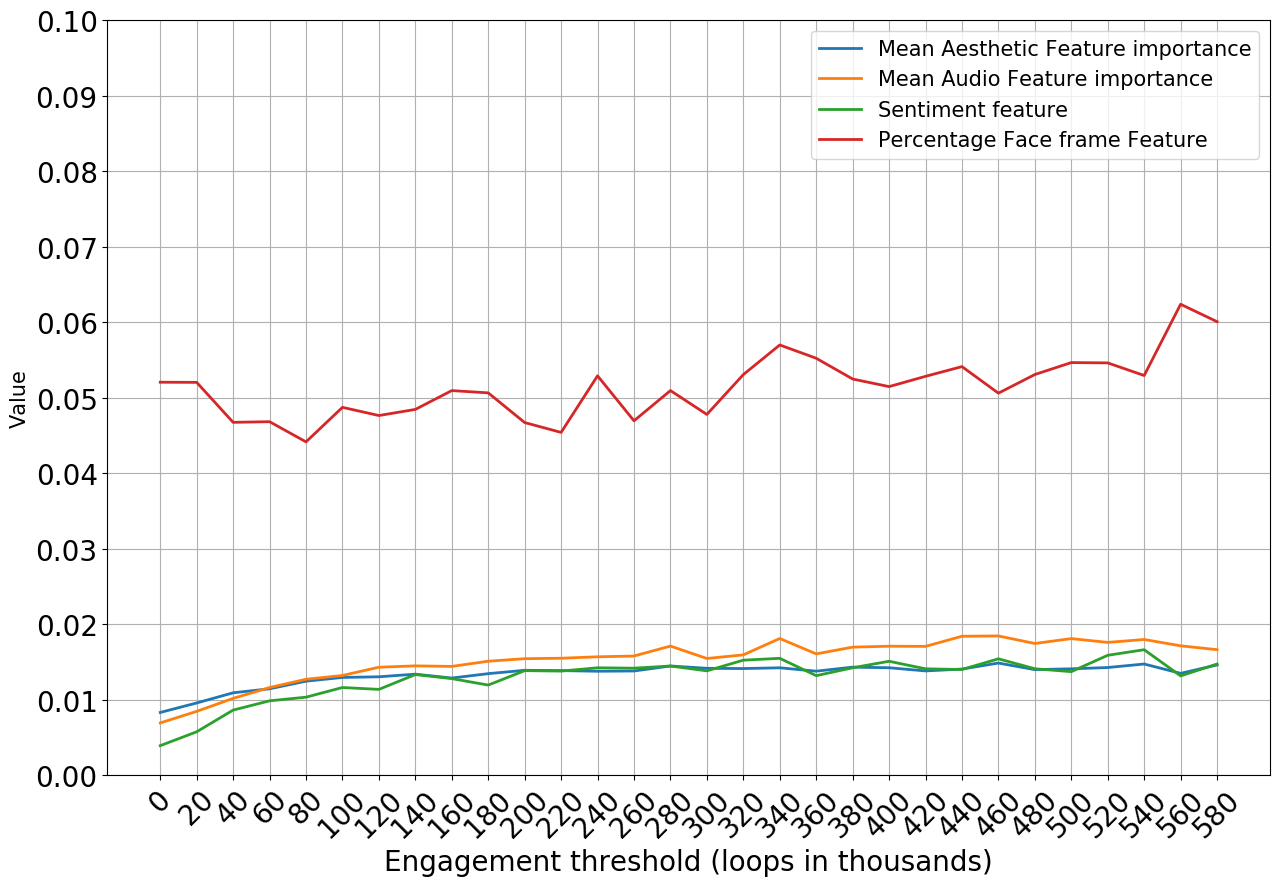
\includegraphics[width=0.5\textwidth, height = 4.5cm]{contentFeatures}
        \label{fig:Feature_importance_content}
    }
    
    \subfloat[ Classifier Performance ]{
        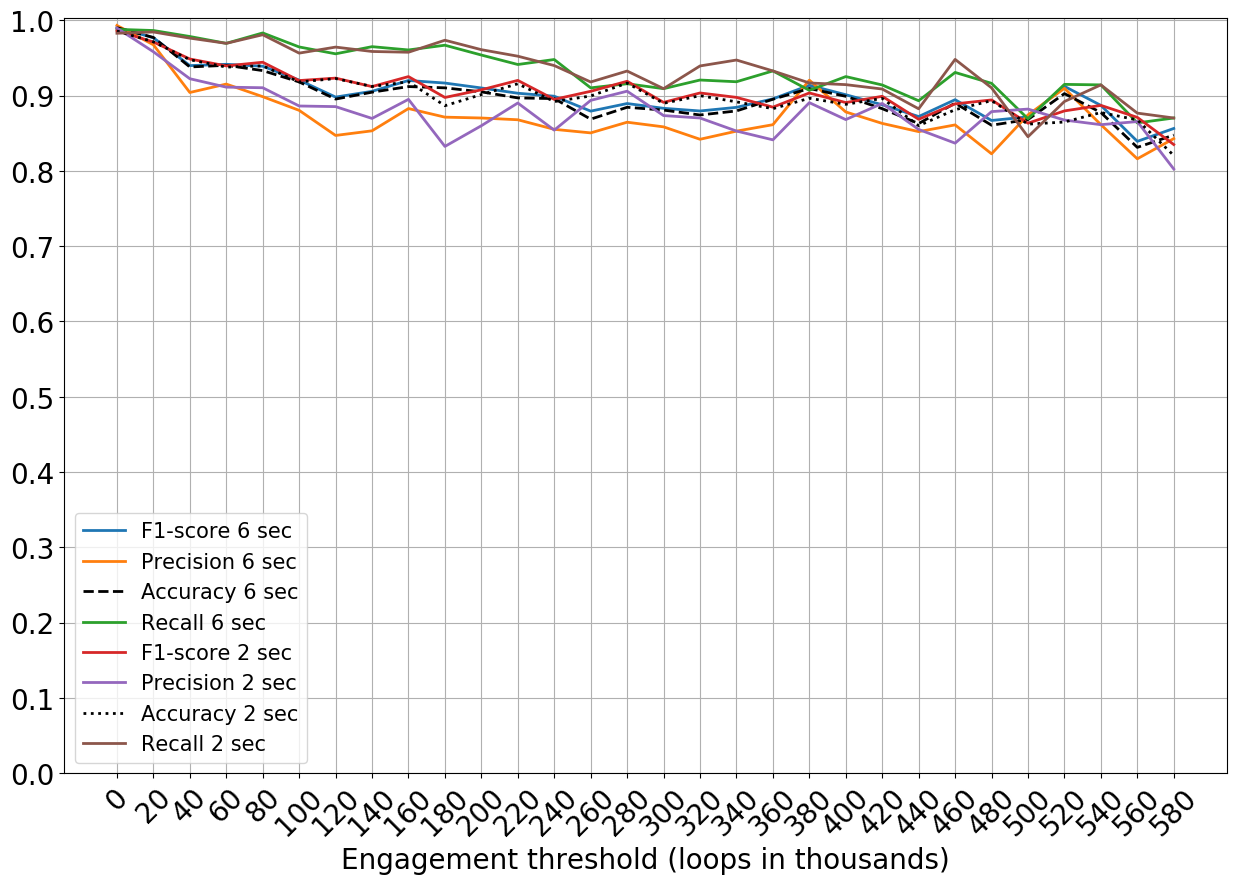
\includegraphics[width=0.5\textwidth, height = 4.5cm]{classifier_accuracy}
        \label{fig:Classifier_performance}
    }
    \caption{ Understanding engagement for different thresholds (min.\ number of loops considered as engaging). Two different classifiers are used, one using quality of the entire micro video (labeled 6 sec), the second measuring quality from only the first two seconds (labeled 2 sec). (a) As threshold becomes higher, content-related factors become as important as social factors (both classifiers). Note that unlike content quality computed from the first 2 seconds (`Content features 2 sec') rather than the entire 6 seconds of the video (`Content features 6 sec'), `social features 6 sec' uses the same feature values as Social Features 2 sec', but the two are plotted separately to show the relative  importance of social features in the 6 second vs 2 second classifier. (b) Amongst content features alone, presence of faces in the video is the single most dominant feature, across all threshold levels (6 second classifier) (c) Both 2 sec and 6 sec classifiers perform similarly across all metrics such as Precision, Recall and F1-score. Performance is high across all engagement thresholds: all metrics are consistently over 0.8 or 0.9.}
    \label{fig:classifier}
\end{figure*}




\begin{figure}[!htb]
    \centering
    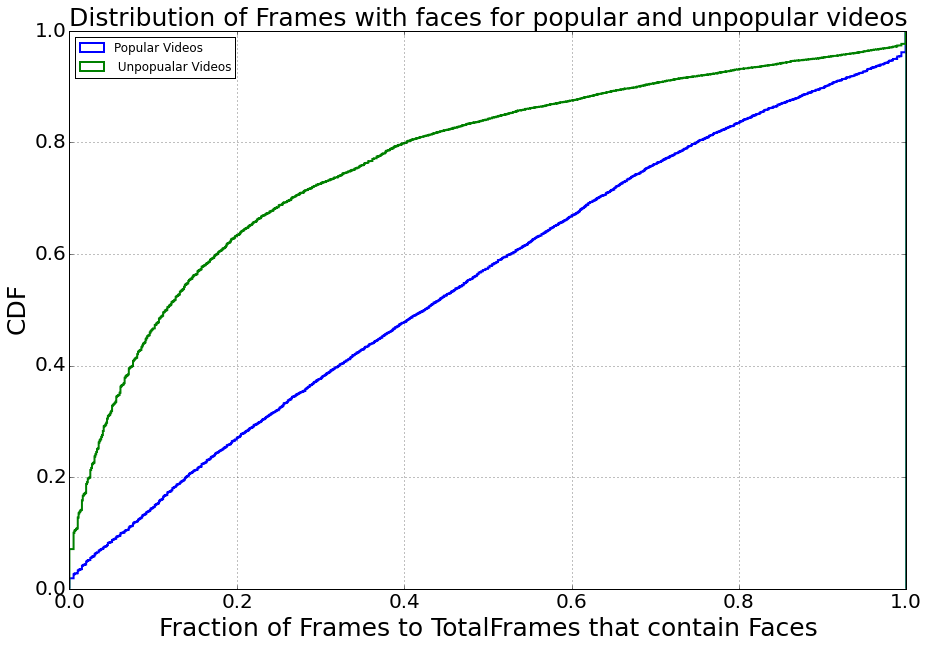
\includegraphics[width=0.6\columnwidth]{FaceCDF}
    \caption{\textsl{ CDF for popular and unpopular videos. The CDF signifies the cumulative distribution of percentages of frames containing faces in a vine video. The observation here is popular videos tend to have higher face percentage than unpopular videos}}
    \label{fig:Face_CDF}
\end{figure}


\section{Primacy of the first seconds}

%Our main observations so far are: \one\ \textbf{RQ1:}Vine micro videos appear to be different from both images (Flickr) and videos (YouTube) and \two\   \textbf{RQw:} content quality features, especially image-related ones (e.g., fraction of faces with frames) become  important for user engagement and popularity metrics. %and \three\ unlike videos where affect (sentiment) plays an important role in user engagement~\cite{bardzell2009understanding,fontanini2016web,eckler2011spreading}\footnote{See also {http://67.222.24.243/wp-content/uploads/2009/03/affect-study-screen-view.pdf} (accessed 24 Oct 2016).}, sentiments conveyed in the video appear to be much less important in Vine. 
Next, we try to understand these findings further by examining the quality of the individual frames of the videos: One way to think about videos is as a sequence of images. With micro videos, this sequence is of course much shorter than in other videos, and we investigate whether this has impact on video quality (\textbf{RQ2}). Our results show a ``primacy of the first seconds'' effect, with quality deteriorating over time and the quality at the beginning is as good a predictor of engagement as quality of the entire video.

\subsection{Image quality deteriorates over time}




Vine videos can be at most 6.5 seconds long. We sample the videos twice every second and represent the whole video as a series of 12-13 static frames. This sampling rate is not too low to miss any considerable frame transitions, neither is it too high to include a lot of mid transition frames. For each sampled frame, we calculate the feature under consideration -- sentiment, percentage of faces, and aesthetic score. To compute the aesthetic score, we extract the 18 aesthetic features described in Table~\ref{tab:Features_table}. for each frame frame. To find an aggregate overall aesthetic score of each frame, we use a weighted sum of all the features (This is possible because all the features are on the same scale), where the weights are calculated to be proportional to the importance of each feature in the classifier designed in the previous section. 


For each video and each feature, we then compute when in the video the feature reached its maximum value. We then divide the videos into two second intervals, essentially dividing the video into its first third, second third and third third. We then ask what proportion of videos had the maximum value of a feature in the first (respectively second and third) third. This procedure tells us when we are likely to find the `best' part of the video. 

\begin{figure}[!htb]
    \centering
    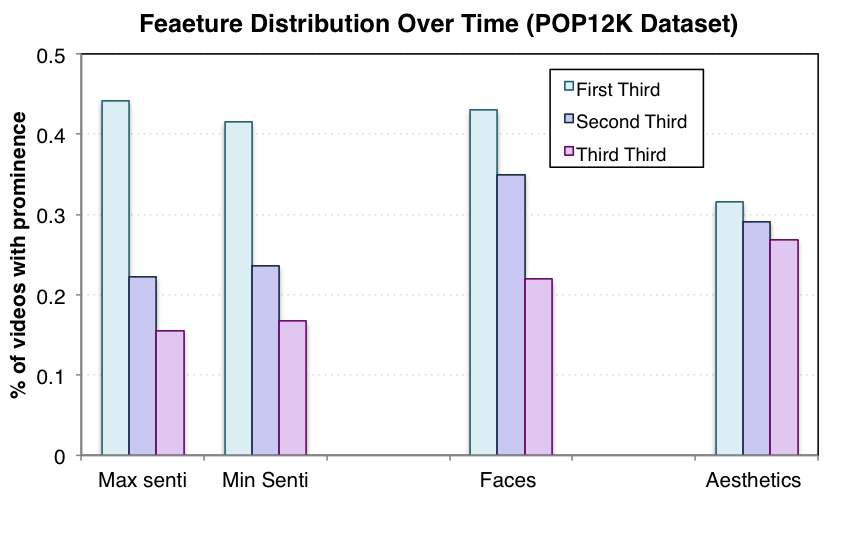
\includegraphics[width=0.7\columnwidth]{ThirdsDistribution.png}
    \caption{\textsl{Evolution of Feature magnitude: The graph shows sharp trend in prevalence of strongest component of a feature in the first one third of the video. The strength decreases progressively for the successive thirds. (Results shown for POP12K dataset. Similar results obtained for ALL120K.)}}
    \label{fig:Face_Thirds}
\end{figure}

Fig.~\ref{fig:Face_Thirds} shows the result for each major category of content-related feature, plotted over both our datasets (ALL120K and POP12K). We observe a general trend where the first third has the maximum (best) value for all features considered. For instance, the best aesthetic score is to be found in the first two seconds. Similarly, the proportion of faces, an important predictor of engagement (Fig.~\ref{fig:Face_CDF}), is also maximum in the first third. 

Note that for sentiment values, the minimum value is just as valid and valuable as the maximum, representing a sad or emotionally dark segment of the movie with negative sentiment, in contrast to a happy segment of the movie with positive sentiment. Therefore, we calculate which third of the movie we find the maximum and minimum sentiment values and plot these separately. In both cases, we find  yet again that the first third of the video has the maximum (minimum) sentiment value for the majority of videos. 

\subsection{Loops and likes are obtained on first sight: Initial seconds predict engagement}
\label{sec:first-seconds}
Collectively, the results above paint a picture where the first seconds of the micro video are highly important in engaging the user. We conjecture that this might be because of the mobile-first nature of Vine: the primary user interface is the Vine app, where users select which videos to watch by scrolling over it. The vine only plays when the user retains focus over the video, and hence the first seconds are likely critical for grabbing user attention and engaging them. 

We next take this result to its logical conclusion, and ask how the classifier developed in the previous section for predicting engagement would work if using only content-related features from the first third of the video rather than from the whole micro video. Following the same methodology as described in the previous sub-section, we develop a series of classifiers for different popularity thresholds, training this time on image content-related features drawn from the first two seconds of the video rather than from across the whole video. The same set of hyper parameters were used as in the previous setting. As shown in Fig.~\ref{fig:Classifier_performance}, the resulting classifiers (labeled 2 sec) perform very similarly to the classifiers developed before (labeled 6 sec). Further, Fig.~\ref{fig:Feature_importance} shows that the relative importance of different features is also nearly identical to the previous results. It should be emphasized that although these results were obtained using loop counts as the metric for user engagement, similar results have also been obtained using reposts (re-vines). 

These results point to a \emph{primacy of the first seconds} effect, whereby the first seconds of a micro video matter as much as the whole video, suggesting that they behave almost like still images in terms of user engagement.


\section{User study}
\label{sec:userstudy}
To complement the data analysis and gain deeper insight into what drives user actions and engagement, we designed an anonymous user study
which captures user behavior when engaging with micro-videos. 

\subsection{Survey methodology}
We initially recruited undergraduate students, obtaining about 33 responses.
Subsequently, we tweeted the survey out to the Official Vine Twitter account and to the accounts of Vine and Instagram users, in order to gain further exposure amongst 
users of these platforms. In all, 115 users responded to our survey. Table \ref{tbl:survey} summarizes the respondents' demography and usage preferences. Most questions asked were to be answered either on a 5-point Likert scale  (Strongly agree to Strongly Disagree), and or in a semantic differential format, with three options to choose from. 
%\footnote{Survey can be found here :  https://goo.gl/forms/lHEea9EzYCyRy3jQ2}.

\begin{table}[hbt]
    \centering
    \begin{tabular}{l|c}
        \thead{Attribute} & \thead{\shortstack{Value}} \\
        \hline
        Male respondents (\%) & 44.2 \\
        Female respondents (\%) & 55.8  \\
        \hline
        Age Demography (\%) &\\
        \hline
        18-24 & 43.4 \\
        25-31 & 34.5 \\
        32-40 & 14.2 \\
        40+    & 8 \\
        \hline
        %		Platforms used (\%) &\\
        %		\hline
        %		Instagram & 67.3 \\
        %		Snapchat stories & 27.4 \\
        %		%Whatsapp stories & 97 \\
        %		Vine & 2 \\
        %		\hline
    \end{tabular}
    \caption{Summary of survey responses}
    \label{tbl:survey}
\end{table}


%We asked users to select the micro-video platforms which the users are most exposed to. Snapchat and Instagram polled highest in the sample population.
%Although Vine polled  low in terms of declared usage, the reason being that Vine was declared to be discontinued as of the date when the survey was conducted\footnote{Moreover our survey was primarily answered by respondents from Europe and Asia, where vine had very limited penetration.}, almost 70\% of users declared to have used Instagram %which also hosts 
%micro videos. Hence this survey can be considered to be a good proxy for understanding ground truth user engagement with micro-videos. 

\subsection{Validation of data-driven results}
To understand engagement with micro-videos and validate the findings that emerged from our analysis of \textbf{RQ1} and \textbf{RQ2}, the survey asked the following 5 questions
to be answered on a 5 level Likert scale (strongly agree - strongly disagree):
\begin{enumerate}
    \small 
    \item [A] I tend to like/comment on videos from friends rather than from strangers
    \item [B] I always form an opinion of a video in the initial few seconds, once the video starts playing
    \item [C] I rarely watch short videos (Snapchats, stories) , all the way to the end.
    %\item [D] I don't really care about the quality of the micro-video or stories, as long as I like the content
    \item [D] I prefer to watch short videos of humans on these platforms. E.g.\ I like to see a person talking/expressing rather than outdoor scenery, or Cats.
\end{enumerate}

Almost 66\% users agreed to question \textbf{A}, which reaffirms the tendency of socially embedded users being able to get high engagement scores. 44\% of users agreed to question \textbf{B} (and further $\approx$ 30\% users were neutral) and 38\% users agreed with statement \textbf{C}, supporting the observed the ``primacy of the first seconds'' effect.
%55\% users agreed to statement \textbf{D}, suggesting a possible reason why . 
Contrary to our findings regarding faces, only 34\% users agreed with statement  \textbf{D} (although a further 39\% remained neutral; thus only a minority 27\% of users disagreed or disagreed strongly). Such result might suggest that for many users, our attraction towards face shapes is innate \cite{slater1998innate} and people do not consciously engage more with faces. %While further study is required to confirm this conjecture, we find that on a sample of 6000 Instagram micro videos, the top 10 percent of videos by popularity had 

\subsection{Understanding what matters to users}
The next part of the survey went beyond confirming the data-driven analysis by asking the respondents how their behaviour changed when it comes to \emph{acting} on a video they engaged with, i.e., when do they like/forward, comment or stop playing the video? 44\% like, comment or share videos only after finishing watching it, and but a sizeable 56\% agreed that they do so in the middle of watching the video itself, or right at the beginning (19\% share at the beginning. 37\% somewhere in the middle); again pointing to the need for capturing users in the initial parts of the video. 

Interestingly, a majority of 55\% of respondents agreed (on a 5 point Likert scale) to the statement: ``I don't really care about the quality of the micro-video or stories, as long as I like the content''. This result, together with the previous answers seems to imply that   the fall off in content quality in the latter parts of micro videos does not negatively impact user engagement. However, users do see a difference between micro videos and ``traditional'' (and older) user generated content platforms such as YouTube: an overwhelming 75\% of respondents rate the production quality of YouTube videos quality as more professional than micro videos.

\section{Discussion and conclusions}
In this work, we took a first look at user engagement with micro videos. Defining engagement in terms of social attention metrics such as likes, revines (reposts) and loop counts, we find that content quality-related features have as strong an influence as social network-based exposure in driving these metrics. Furthermore, the quality of the first couple of seconds is higher than the quality of subsequent seconds, and can predict whether a micro video will be engaging or not, just as well as looking at the quality of the entire video. We further conduct a user study to understand ground-truth user behavior when it comes to micro-videos. The study suggests that users tend to make quick opinions regarding micro-videos and engage with them almost in an image-like fashion, where they may begin but not finish  watching the short 5-10 second long video. 
%This `primacy of the first seconds' effect suggests the observation that  micro videos are somewhat closer to user-generated images rather than user-generated videos, which we corroborated by comparing popular micro videos on Vine  to popular images on Flickr and viral videos on YouTube.
On a big picture scale, we show that attention budgets are quantifiable if we have a large enough user engagement data. Drawing back to the DIKW pyramid, the wisdom gathered from this knowledge extraction pipeline can imply several things.
\begin{enumerate}
    \item Advertisements on the Web are driven by social attention metrics. Therefore advertisers need to know and adjust their strategies based on the insight that user attention is driven to a large extent by the initial seconds. Although  video ads do not appear to be common in today's micro videos, how to place ads that grab user attention within a short duration of time will be a problem that is interesting both from a research and a business perspective. 
    \item A possible reason for the deterioration of image quality is that it may be difficult to maintain image composition, focus etc using a mobile phone camera with moving subjects. Novel UI and multimedia techniques that can help correct for such quality deterioration could greatly help micro video creators -- and also represent a second promising direction for further study. 
    \item Recently, several micro video platforms have started extending the duration of micro videos. Although the wisdom of longer micro videos without appropriate editing tools has been questioned\footnote{\scriptsize http://www.theverge.com/2013/6/20/4448906/video-on-instagram-hands-on-photos-and-video}, from a research perspective it would be interesting to study how user behavior and engagement changes as longer micro videos become more common place. Interestingly, we find that in a small sample of about 6000 Instagram videos (where the maximum permitted duration is 60 seconds), users continue to prefer shorter videos, with 70\% of videos less than 20 seconds long, and the median duration at just under 15 seconds. Such user preferences can and should be considered as the micro video format evolves further on different platforms.
\end{enumerate}

More generally, in this work we considered user engagement as a single dimension of perception driven process. We acknowledge that user engagement is a very subjective notion, impacted by different factors including user location, habits, gender, visual preferences. In  future work, we plan to explore how such different user sub-cultures perceive and engage with micro videos, following recent works from the Multimedia community studying the impact of culture in subjective image perception \cite{jou2015visual}.








